% !TEX root = diplomarbeit.tex
\chapter{Positionierung}
\renewcommand{\kapitelautor}{Autor: Christina Bornberg}

%%%%%%%%%%%%%%%%%%%%%%%%%%%%%%%%%%%%%%%%%%%%%%%%%%%%%%%%%%%%%%%%%%%%%%%%%%%%%%%
\section{Allgemeine technische Planung}

    \subsection{Allgemein}
    Um eine Positionsbestimmung durchzuführen, wird ein Trackingsystem benötigt.
    Es gibt mehrere Verfahren\cite{PositionAllg}, um ein Objekt zu tracken: 
    \begin{itemize}
    \item Mechanische Systeme, umgesetzt mit einer mechanischen Verbindung
    \item Elektromagnetisches Tracking, umgesetzt mit elektromagnetischen Wellen
    \item Akustisches Tracking, umgesetzt mit akustischen Wellen
    \item Optisches Tracking, umgesetzt mit elektromagnetischen Wellen
    \item Inertial Tracking, umgesetzt mit Beschleunigungsmessern und Gyroskopen
    \item Hybride Ansätze, umgesetzt mit Kombinationen, die mehrere Systeme vereinen
    \end{itemize}
    Elektromagnetische, optische und akustische Verfahren werden in späteren Abschnitten genauer behandelt.

    \subsection{Anwendung}
    Indoor Positionierungssysteme werden derzeit vor allem zur Objekterkennung, im Umweltmonitoring, über das Detektieren von Bränden in Gebäuden, bis hin zum Einsatz in der Logistik, verwendet. Da es sehr viele unterschiedliche Anwendungsgebiete\cite{posAnwendung} gibt, werden unterschiedliche Methoden verwendet. 

    \subsection{Eigenschaften der Positionsbestimmung}
    Ein Positionierungssystem kann verschiedene Arten von Informationsdaten\cite{pos_eigenschaften} aufweisen. 

    \subsection*{Physische und symbolische Positionierung}
    Die \textbf{physische Positionierung} ist eine exakte Position, die zum Beispiel in einem Koordinatensystem, meist in 2-D oder 3-D Karten, bestimmt wird. Längen- und Breitengrade spielen dabei eine wichtige Rolle.\\
    \textbf{Symbolische Positionierung} ist die abstrakte Beschreibung eines Ortes, sie wird sprachlich beschrieben, beispielsweise Küche, Garten, Dachboden.\\
    Eine physikalische Position kann auch symbolisch beschrieben werden.

    \subsection*{Relative und absolute Positionierung}
    Autor: Lucas Ullrich\\

    \textbf{Absolute Positionsmessung}\\
    Hier wird die Position von einem gleichbleibenden Bezugspunkt aus gemessen. Dabei ist ein konstanter Referenzpunkt wichtig.
    Verändert sich dieser oder kann die Distanz nicht genau gemessen werden, ist die Messung unbrauchbar.

    Für eine absolute Positionsmessung bieten sich diverse Triangulationsverfahren an, diese sind ausgesprochen rechenaufwändig und benötigen meist eine sehr genaue Laufzeitmessung.
    Für die Triangulation können die unterschiedlichsten Signale verwendet werden, am gängigsten sind jedoch jene die mit elektromagnetischen Wellen arbeiten,
    zum Beispiel WLAN, Bluetooth. Dies bedeutet, dass sich die Signale mit Lichtgeschwindigkeit ausbreiten.

    Bei einer Messung derart schneller Signale muss ein hoher Aufwand betrieben werden um eine Messgenauigkeit von einigen cm zu erzielen.

    Eine weitere Herausforderung sind Hindernisse wie Mauern. Hier muss ständig berücksichtigt werden wo ein Objekt steht und ob der geplante Weg überhaupt frei ist.

    \textbf{Relative Positionsmessung}\\
    Hier wird die Position von einem wechselnden Punkt aus gemessen. Um hier eine Positionierung im Raum ermöglichen zu können,
    ist es erforderlich immer zu einem bestimmten Punkt zu messen. Ein Wechsel dieses Punktes ist jedoch möglich,
    deshalb muss auch die Position der Punkte im Raum bekannt sein. Ist die Zielposition im Raum bekannt, kann zu dieser hin navigiert werden.
    Auch hier muss wie bei einer absoluten Positionsmessung auf Hindernisse geachtet werden.

    Die zweite Möglichkeit ist, dass eine bestimmte Route bekannt ist und sich das zu positionierende Objekt nur in einem bestimmten Bereich um diese Route bewegt.
    Wird bei der Positionierung der Route bereits auf Hindernisse geachtet müssen diese im Anschluss nicht mehr zwingend beachtet werden.

    \subsection*{Selbst- und fernortende Lokalisierungstechniken}
    Lokalisierungstechniken können weiter als selbstortend oder fernortend (self­positioning/remote­positioning) klassifiziert werden. Beim optischen Tracking werden die beiden Varianten Inside-out und Outside-in genannt.\\
    Beim \textbf{selbstortenden Positionierungssystem} bekommt der mobile, bewegliche Empfänger die Daten von verschiedenen Sendern, die sich auf bekannten Positionen befinden. Die Lokalisation des Empfängers wird durch die gemessenen Signale ermittelt. Das Objekt kann sich selbst orten, es ist kein Netzwerk notwendig.\\
    Ein \textbf{fernortendes Positionierungssystem} besteht aus einem mobilen, beweglichen Sender und stationären, unbeweglichen Empfängern. Die Messdaten aller Empfänger werden gesammelt und die Position des Senders wird in der Zentrale berechnet. Hier ist ein Netzwerk notwendig, sämtliche Berechnungen werden durch eine zentrale Instanz ausgeführt.

    \begin{figure}[H]
      \begin{centering}   
        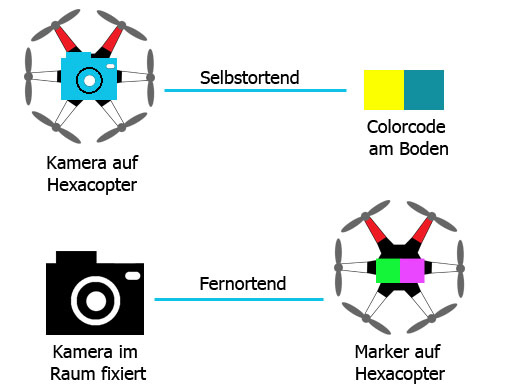
\includegraphics[width = 0.7\textwidth]{Bilder/bor_selbst_fern}}
      \par\end{centering}
      \caption{Selbstortende und fernortende Lokalisierung}
      \label{SelbstundFernortend}
    \end{figure}

    \subsection*{Genauigkeit}
    Die Genauigkeit gibt an, wie sehr sich gemessene und tatsächliche Position unterscheiden.

    \subsection*{Skalierung}
    Hierbei gibt es mehrere Faktoren, beispielsweise die Anzahl der zu trackenden Objekte, die Reichweite und die benötigte Zeit.

    \subsection*{Kosten}
    Hier gibt es Kosten im Bereich der Anschaffung des Systems und Kosten während des Betriebs.

    \subsection*{Limitierung}
    Unter Limitierung fallen Einschränkungen und Störfaktoren. Manche Systeme haben besondere Ansprüche an ihre Umgebung.

    \subsection{Elektromagnetische Verfahren}
    Elektromagnetische Wellen bestehen aus einer Kombination von elektrischen und magnetischen Wellen. Das für das menschliche Auge sichtbare Spektrum nennt man Licht. Optische Verfahren sind in einem der folgenden Abschnitte erklärt. Weitere Beispiele sind Ultraviolett, Infrarot, Radiowellen, Mikrowellen und Röntgenstrahlung.

    Verfahren zur Positionsbestimmung mittels Signal\cite{pos_signal_2} \cite{pos_signal_4}: 

    \subsection*{Lateration}
    Bei der Lateration wird die Position mit Hilfe der Entfernungsmessung bestimmt.
    Techniken der Lateration sind TOA (Time Of Arrival) und TDOA (Time Difference Of Arrival).\\
    
    Bei \textbf{TOA} werden Signale in Laufzeit gemessen. Durch die Zeitdifferenz zwischen Sender und Empfänger, kann die Entfernung mithilfe der Information, wie schnell sich das Signal fortbewegt, errechnet werden. Da sich elektromagnetische Wellen in Lichtgeschwindigkeit ausbreiten, ist die zu messende Laufzeit sehr gering. Ultraschallsignale bewegen sich vergleichsweise langsam, dies vereinfacht die Zeitmessung.
    Um schlussendlich die Position zu bestimmen, werden drei Basisstationen benötigt, die jeweils eine Entfernungsmessung zum mobilen Objekt durchführen. Durch die drei Entfernungen kann mittels Trilateration die Position berechnet werden. Meist ist eine vierte Basisstation nötig um die Synchronisation der Uhr der mobilen Station mit jener der Basisstationen zu ermöglichen.

    \textbf{TDOA} basiert auf der Laufzeitdifferenzmessung.
    Die mobile Station sendet einen Zeitstempel an drei Basisstationen. Durch die Differenz der Laufzeiten, kann die Position ebenfalls mittels Trilateration bestimmt werden.

    \subsection*{Angulation}
    Bei der Angulation wird die Position durch die Bestimmung von Winkeln ermittelt. \\
    \textbf{AOA} (Angel of Arrival) wird mittels Berechnung des Einfallswinkels auf ein Antennenarray umgesetzt. Bei dieser Technik werden mindestens 2 Basisstationen benötigt. Mit den Einfallswinkeln der empfangenen Signale kann die Position durch Triangulation festgestellt werden. Die Winkelbeziehungen eines Dreiecks werden dafür verwendet.
    Bei dieser Technik muss keine Synchronisation durchgeführt werden. Der Nachteil ist die benötigte komplexe Hardware.

    \subsection*{Scene Analysis}
    Bei der Szenenanalyse werden Umgebungsparameter erfasst und ausgewertet.\\
    Für die Technik \textbf{Fingerprint} werden Signalstärken gemessen und als Fingerprint in einer Datenbank abgespeichert. Die Position wird dann durch den Vergleich von Fingerprints mit der Signalstärke, die bei der aktuellen Position gemessen wird, herausgefunden.
    \subsection*{Proximity}
    Für das Verfahren Proximity wird die physische Nähe genutzt.
    Hier gibt es die Technik COO (cell of origin). \\
    Bei \textbf{COO} gibt es Basisstationen, mit bekannter Position. Die mobile Station verbindet sich mit der nächstgelegenen Basisstation. Wenn die mobile Station von mehreren Basisstationen erkannt wird, wird die Signalstärke beachtet. Diese Methode ist sehr ungenau.

    \subsection{Elektromagnetische Technologien}
    \subsection*{GPS (Global Positioning System)}
    GPS ist ein satellitengestütztes Navigationssystem, das Ende der 1980er-Jahre zur globalen Positionsbestimmung entwickelt wurde. Die Nachteile des Systems sind der schlechte Empfang der Satellitensignale für indoor-Anwendungen.
    \subsection*{RFID (Radio-Frequency IDentification)}
    RFID bezeichnet eine Technologie für Sender-Empfänger-Systeme zum automatischen und berührungslosen Identifizieren und Lokalisieren von Objekten mit Radiowellen. Ein RFID-System besteht aus einem Transponder, der sich am oder im Objekt befindet und einen kennzeichnenden Code enthält, sowie einem Lesegerät zum Auslesen dieser Kennung.
    \subsection*{WPS (WLAN Positioning System)}
    WPS ist ein indoor Positionierungssystem, das auf WLAN basiert. Durch sogenannte  Access Points (drahtloser Zugangspunkt), wird die Entfernung zu Endgeräten bestimmt. Durch drei Access Points kann mittels Dreiecksmethode, die Position des Endgeräts ermittelt werden.

    \subsection{Akustische Verfahren}
    \subsection*{Puls-Echo-Methode}
    Die Puls-Echo-Methode\cite{akustischeverfahren} ist auch als TOF (Time Of Flight) bekannt.
    Das Messprinzip erweist sich als sehr einfach. Ein Ultraschallsensor sendet einen, durch einen kurzen Spannungsimpuls erzeugten, Wellenzug aus, der daraufhin von einem Objekt reflektiert wird und schlussendlich zum Sender des Sensors gelangt. Die Entfernung, zwischen Sensor und zu erkennendem Objekt, kann nun aus der Laufzeit des Ultraschallsignals berechnet werden. 
    \subsection*{Phasenverschiebung}
    Bei der Phasenverschiebung\cite{akustischeverfahren} wird ein kontinuierliches Ultraschallsignal gesendet. Nachdem die Welle reflektiert wurde, wird sie ebenfalls von einem Empfänger aufgenommen. Die Phasenverschiebung kann nun zwischen gesendetem Referenzsignal und empfangenem Signal gemessen werden. Mithilfe dieser Information ist es möglich Laufzeit und zurückgelegte Distanz abzuleiten. 

    \subsection{Akustische Technologien}
    \subsection*{Ultraschall}
    Ein Ultraschallsensor ist Sender und Empfänger in einem. Das System basiert auf der Zeitdifferenzmessung. Er sendet ein Signal, dieses wird reflektiert und anschließend empfängt der Sensor sein eigenes Echo. Mithilfe der Ausbreitungsgeschwindigkeit akustischer Wellen, ist es möglich Entfernungen zu messen. Die Zeit, die ein Signal zum zu messenden Objekt und wieder zurück braucht, nennt man Laufzeit, da die Strecke doppelt gemessen wird, wird die Zeit halbiert.

    \subsection{Optische Verfahren}
    Maschinelles Sehen (machine vision)\cite{machinevision} \cite{machinevision2} beschreibt die Fähigkeit eines Computers zu sehen.
    Für einen Menschen ist es einfach, Objekte auf einem Bild zu erkennen, für Computer besteht ein Bild jedoch aus Daten, die die Graustufe beziehungsweise Farbe jedes einzelnen Pixels angeben, was die Möglichkeit des "Bildverstehens" erschwert.
    Die Auswertung erfolgt mathematisch, weswegen die Stärken von maschinellem Sehen im Bereich der Bestimmung von Farben und Graustufen, sowie der Entfernungsmessung liegen. Weiters können Maschinen, im Gegensatz zum menschlichen Auge, Infrarotlicht, Ultraviolettes Licht und Röngtenstrahlen wahrnehmen.

    Es wird zwischen Objekt Erkennung (detection)\cite{obj_det_trak} und Verfolgung (tracking) unterschieden. Erkennung bezieht sich auf ein einzelnes Objekt, das in einem Bild erkannt wird. Bei der Verfolgung werden ein oder mehrere Objekte über eine Sequenz von Bildern erkannt und somit verfolgt.
    
    \subsubsection{Bildverarbeitung}
    Die Bildverarbeitung \cite{Bildverarbeitung2} besteht aus einer Reihe von Schritten, je nach Anwendung werden dabei manche ausgelassen.
    Der Beginn besteht aus der Bildvorverarbeitung, bei der das Bild optisch verbessert wird. Daraufhin folgt die Bildanalyse, die aus den Schritten besteht: 
    \begin{itemize}
    \item Segmentierung, in der das Bild in Bereiche aufgeteilt wird
    \item Merkmalsextraktion, bei der beispielsweise Kanten erkannt werden
    \item Klassifizierung, bei der das Bild Klassen zugewiesen wird
    \end{itemize}

    \subsubsection{Segmentierung}
    Beim Segmentieren teilt man ein Bild in Segmente mit gleichen Merkmalen auf.

    \subsection*{Pixelorienterte Segmentierung}
    Pixelorientierte Segmentierung\cite{Seg_punkt} wird auch punktorientierte Segmentierung genannt. Sie basiert auf den lokalen Pixelinformationen, in Abhängigkeit der Grauwerte.

    \textbf{Thresholding}\\
    Beim Thresholding, auch Schwellenwertverfahren genannt, werden Bildpunkte verschiedenen Gruppen zugeordnet. Da es eine histogrammbasierte Segmentierung ist, wird das zu segmentierende Bild binärisiert, das bedeutet, dass jedes Pixel entweder schwarz oder weiß eingefärbt wird. Dies wird durch den Vergleich des Grauwerts oder einem anderen eindimensionalen Merkmal mit einem Schwellwert, erreicht. Der Grauwert bezieht sich nur auf die Helligkeit der Pixel, Informationen zur Farbe werden dabei ignoriert. Da dieses Verfahren bei jedem einzelnen Pixel angewendet wird, gehört es zur pixelorientierten Segmentierung. Diese Technik benötigt wenig Rechenleistung, weshalb es in Echtzeitsystemen angewendet werden kann.

    \subsection*{Modellbasierte Segmentierung}
    Modelle, bestehend aus Pixelgruppen, werden auf Instanzen geprüft. Einfache Modelle werden mittels Template Matching oder der Hough-Transformation analysiert. 

    \textbf{Templatematching}\\
    Um Objekte in Bildern zu finden, müssen Information zu Struktur, Form oder Farbe vorliegen. Templates,\cite{Seg_modell} in denen diese Informationen enthalten sind, werden mit dem Bild verglichen. Anschließend wird die Region im Bild gesucht, die die größte Ähnlichkeit aufweist.

    \textbf{Hough-Transformation}\\
    Durch die Hough-Transformation\cite{Seg_modell} können anhand der Anzahl der Pixel, die von der gesuchten Form überdeckt werden, geometrische Objekte, wie beispielsweise Kreise, erkannt werden. Dieses Verfahren ist sehr robust, da es auch auf verrauschten Bildern unvollständige oder teils verdeckte Objekte erkennt.


    \subsection*{Regionenorientierte Segmentierung}
    Hier werden benachbarte Pixel\cite{Seg_region} auf Gleichheit zum Startpixel geprüft.

    \textbf{Region Growing}\\
    Bei diesem Verfahren geht man von einem Startpixel, beziehungsweise Seed-Point aus, dieses kann entweder vom Menschen selbst oder vom Computer gewählt werden. Dieses wird mit benachbarten Pixeln auf ähnliche Eigenschaften verglichen. Wenn diese Pixel genügend Ähnlichkeit aufweisen, werden sie zu einer sogenannten Region hinzugefügt, andernfalls wird das jeweilige Pixel ignoriert. Die Technologie kann in verrauschten Bildern angewendet werden.

    \subsection*{Texturorientierte Segmentierung}
    Da sich Objekte oft durch eine einheitliche Struktur auszeichnen, versucht dieses Verfahren dies als Homogenitätskriterium zu verwenden. Texturorientierte Segmentierung\cite{Seg_textur} wird meist zur Unterstützung anderer Methoden verwendet. 

    \textbf{Co-Occurrence-Matrizen}\\
    Um eine Texturanalyse durchzuführen, kann die Co-Occurrence-Matrix\cite{seg_coocc}, auch Grauwertübergangsmatrix genannt, verwendet werden. 
    Bei dieser Matrix werden die Grauwertverhältnisse der Umgebung eines Pixels beschrieben.

    \subsubsection{Merkmalsextraktion}
    Bei diesem Schritt sollen Merkmale wie Kanten und Ecken erkannt werden.

    \textbf{Kantendetektion}\\
    Im menschlichen Sehen, haben Kanten eine wichtige Bedeutung, durch sie kann ein Bild beinahe vollständig nachgebildet werden. Es gibt einige Verfahren um die Erkennung der Objektgrenzen durchzuführen. Es wird dabei zwischen physikalischen Kanten, die durch inhomogene Intensitätswerte bei Verläufen erkannt werden und Pseudokanten, die durch Schatten Kanten erzeugen, die nicht existieren, unterschieden.
    Das Verfahren besteht grundsätzlich aus 3 Schritten:
    \begin{itemize}
        \item Um den Intensitäts-Gradienten zu erzeugen, wird eine Maske angewendet.
        \item Nennenswerte Gradienten werden mittels Thresholding selektiert.
        \item Durch verschiedene Operationen und Algorithmen entstehen, mittels errechneter Daten, Kanten.
    \end{itemize}
    Die Verfahren können in zwei Kategorien eingeteilt werden.
    \begin{itemize}
        \item \textbf{1. Ableitung}\\
        Hierfür können Sobel Operator, Laplace-Filter, Canny Algorithmus verwendet werden.
        \item \textbf{2. Ableitung}\\
        Für die 2. Ableitung kommt beispielsweise der Sombrerofilter, auch Laplace of Gaussian Operator oder Marr-Hildreth-Operator genannt, zum Einsatz.
    \end{itemize}

    \textbf{Eckendetektion}\\
    Ecken sind Punkte, in denen zwei Kanten enden und sind somit Objektabschlüsse. Sie sind ebenfalls wichtige Merkmale in einem Bild und können durch Gradienten oder Morphologie erkannt werden. Um die Eckendetektion\cite{Bildverarbeitung} durchzuführen, können beispielsweise Moravec´s Corner Detector und Harris Corner Detector verwendet werden.

    \subsubsection{Klassifikation}
    Klassifizieren\cite{Bildverarbeitung} ist das Zusammenfassen von Objekten zu einer Gruppe, Klasse beziehungsweise Kategorie. Hier gibt es beispielsweise die Klassifikation nach Farbe, Kontrast, Segmentgröße, Form oder Textur. Durch die Klassifikation soll das Erkennen von Zusammenhängen verbessert werden. Ein Objekt, bei dem alle relevanten Eigenschaften vorliegen, kann korrekt klassifiziert werden. Da in den meisten Fällen nicht alle Informationen vorliegen, wird eine Klassifizierung anhand eines Merkmalvektors, der aus einer Reihe passender Merkmale entsteht, durchgeführt. 

    \subsection{Optische Technologien}
    \subsection*{Pixy CMUcam5}
    Die Pixy CMUcam5\cite{Pixy} ist ein optisches Trackingsystem. Das Kameramodul ist in der Lage, Objekte in 7 verschiedenen Farben zu scannen, diese zu speichern und wiederzuerkennen. Daten über die Höhe und die Breite, sowie die x- und y-Position des getrackten Objektes innerhalb des Frames werden ausgegeben. Bei sogenannten Colorcodes, die sich aus zwei oder mehrfarbigen Objekten ergeben, kann die Rotation des Objektes ebenfalls ermittelt werden.

    \textbf{CMVision}\\
    Color Machine Vision\cite{Pixy_Verfahren} \cite{Pixy_Verfahren2}, ist ähnlich dem Algorithmus der Pixy. Es ist ein Echtzeitsystem, das mit dem Farbmodell YUV umgesetzt wird. Das Y steht für die Lichtstärke pro Fläche, U und V geben den Farbanteil an. Der Vorgang beginnt mit einer Farbraumtransformation. Als Segmentierungsmethode wird Thresholding angewendet. Regionen werden verbunden und entnommen. Am Ende werden die Regionen zusammengefasst.  

    \subsection*{Vicon}
    Vicon\cite{Vicon} ist ein System, das mit dem Trackingverfahren Motion Capture (Bewegungserfassung) arbeitet.
    Mehrere Kameras werden in einem Raum verteilt. Jede Kamera besitzt einen Infrarotfilter und Infrarot-LEDs. Die Lampen senden infrarotes Licht aus, dieses wird an Markern, die sich auf dem zu trackenden Objekt befinden, reflektiert. Mithilfe einer Software kann dadurch eine dreidimensionale Karte erstellt werden.
    

  \section{Konzepte}

    \subsection{Aufgabenstellung}
    Die verschiedenen Positionierungsarten wurden verwendet, um Konzepte für die Navigation zu entwickeln. Das Ziel ist ein autonomer Flug in einem Raum.

    \subsection{Elektromagnetisches Tracking: Fernortend}

      \subsection*{Tracking mittels Time of Arival}
      Mithilfe der Laufzeitmessung können Objekte, die mit einem Empfänger ausgestattet sind, geortet werden. Dafür wird die Zeit, die ein Signal vom Sender zum Empfänger benötigt gemessen. Das Signal ist eine elektromagnetische Welle, die sich im Vakuum in Lichtgeschwindigkeit ausbreitet. Die gemessene Laufzeit wird mit der Lichtgeschwindigkeit multipliziert, damit kann die Entfernung berechnet werden. Für diese Variante benötigt man eine sehr hohe Zeit-Messgenauigkeit.

      Bei diesem Konzept, soll durch die Benützung sogenannter Pseudolites (gefälschte Satelliten) eine Art lokales GPS erschaffen werden.

      Das System besteht aus 3 Sendern, die Signale schicken und einem Empfänger, der sich im Hexacopter befindet.
      Durch das Senden eines Signals von jedem Pseudolite zum Empfänger, können 3 Distanzen berechnet werden.
      Aus diesen 3 Distanzen und der bekannten Koordinaten der Pseudolites, wird die augenblickliche Position mittels Trilateration\cite{pos_signal_2} des Hexacopters berechnet.

\[
      Distanz 1 = (x1 - x)^{2} + (y1 - y)^{2} + (z1 - z)^{2}
\]
\[
      Distanz 2 = (x2 - x)^{2} + (y2 - y)^{2} + (z2 - z)^{2}
\]
\[
      Distanz 3 = (x3 - x)^{2} + (y3 - y)^{2} + (z3 - z)^{2}
\]

      Distanz ... ist die durchgeführte Messung\\
      x1, y1, ... z2, z3 ... sind die statischen Koordinaten der Pseudolites \\
      x, y, z ... werden durch die Lösung dieses quadratischen Gleichungssystems ermittelt \\

      Beim Lösen der Gleichung erhält man zwei Schnittpunkte. Dies ergibt sich aus der logischen Schlussfolgerung, dass die Oberflächen dreier verschmolzener Kugeln zwei Schnittpunkte haben.
      Wenn die Pseudolites am Boden angebracht werden, liegt eine der beiden Lösungen oberhalb und die zweite Lösung unterhalb des Bodens, womit man einfacher Weise, die Lösung mit der negativen Z-Koordinate ausschließen kann.

    \subsection{Optisches Tracking: Fernortend}
    Aufgrund der Komplexität signalbasierter Verfahren, die ihre Position mittels elektromagnetischer Wellen bestimmen, werden hier Konzepte, die durch eine oder mehrere Kameras umgesetzt werden können, näher beschrieben. Beim optischen Tracking mit Markern wird mit Kameras gearbeitet, welche aktive (Signal emittierende) oder passive Marker an den zu erfassenden Personen oder Gegenständen verfolgen.

  \subsection*{Kamerasystem im Raum}
  Bei einem Raum, in dem Kameras verteilt sind, spricht man von einem fernortenden Positionierungssystem.
  Sowohl Tische und Kreuzungen als auch der Hexacopter sind mit Markern versehen. Die einzelnen Komponenten werden vom Kamerasystem erfasst und anschließend wird eine Karte erstellt. Diese Karte besitzt, wie ein Koordinatensystem Längen und Breitengrade.
  Um den Weg vom Stützpunkt zum gewünschten Tisch zu finden, muss der Hexacopter eine Route wählen. Diese bestimmt er mithilfe der Daten, wodurch er sich selbst, Kreuzungen und Tische findet. Da das System die Position des Hexacopters trackt, kann kontrolliert werden, ob dieser sich auf dem richtigen Weg befindet. Die Position der einzelnen Komponenten kann, wie bei signalbasierten Verfahren, mittels Triangulation berechnet werden.

  \subsection{Optisches Tracking: Selbstortend}
  Selbstortende, optische Positionierungssysteme sind vergleichsweise kostengünstig. Der Anschaffungspreis beschränkt sich auf eine Kamera, einen Mikrocontroller und Farbobjekte. Die Auswertung erfolgt am Hexacopter, weswegen kein extra Netzwerk benötigt wird.

  \subsection*{Linien}
  Bei einem selbstortenden Positionierungssystem sind Sensoren auf dem sich bewegenden Objekt angebracht.
  Eine am Hexacopter fixierte Kamera trackt Linien, die sich am Boden befinden. Der Hexacopter soll einer einfarbigen Linie folgen, bis er zu einer Kreuzung kommt, nun ist seine Aufgabe jeweils die nächste Linie bis zum Erreichen des Ziels zu finden. Der Vorteil dieser Strategie ist es, dass der Hexacopter eine Linie eher schwer verlieren wird, das gewählte Kamerasystem Pixy, kann jedoch nur Farbobjekte tracken.

  \subsection*{Ein Farbcode pro Wegabschnitt}
  Durch die Verwendung der Pixy CMUCam5 ergibt sich die Möglichkeit, Farbobjekte, die eine oder mehrere Farben aufweisen, zu scannen.
  Das Kamerasystem besitzt die Fähigkeit sieben unterschiedliche Farben zu erkennen, diese können vom Administrator selbst festgelegt werden. Da die Lichtverhältnisse sich nicht stark ändern sollten, ist es optimal, die Farben in dem Raum, in dem das System verwendet wird, abzuspeichern.

  Bei diesem Konzept bekommt der Mikrocontroller Informationen zu den Farbobjekten pro Wegabschnitt. Vom Start bis zur ersten Kreuzung verwendet er eine Farbinformation, die aus einem Colorcode besteht. Jedes Farbobjekt auf diesem Weg hat dieselben zwei Farben. Durch diese Technik hat der Administrator des Systems weniger Aufwand. Hierbei kann es aber zu Komplikationen führen. Der Hexacopter erkennt beispielsweise einen der bereits passierten Farbcodes und bezieht die Position auf diesen. Die relative Position beschränkt sich bei dieser Variante auf den Wegabschnitt.

    \begin{figure}[H]
      \begin{centering}
        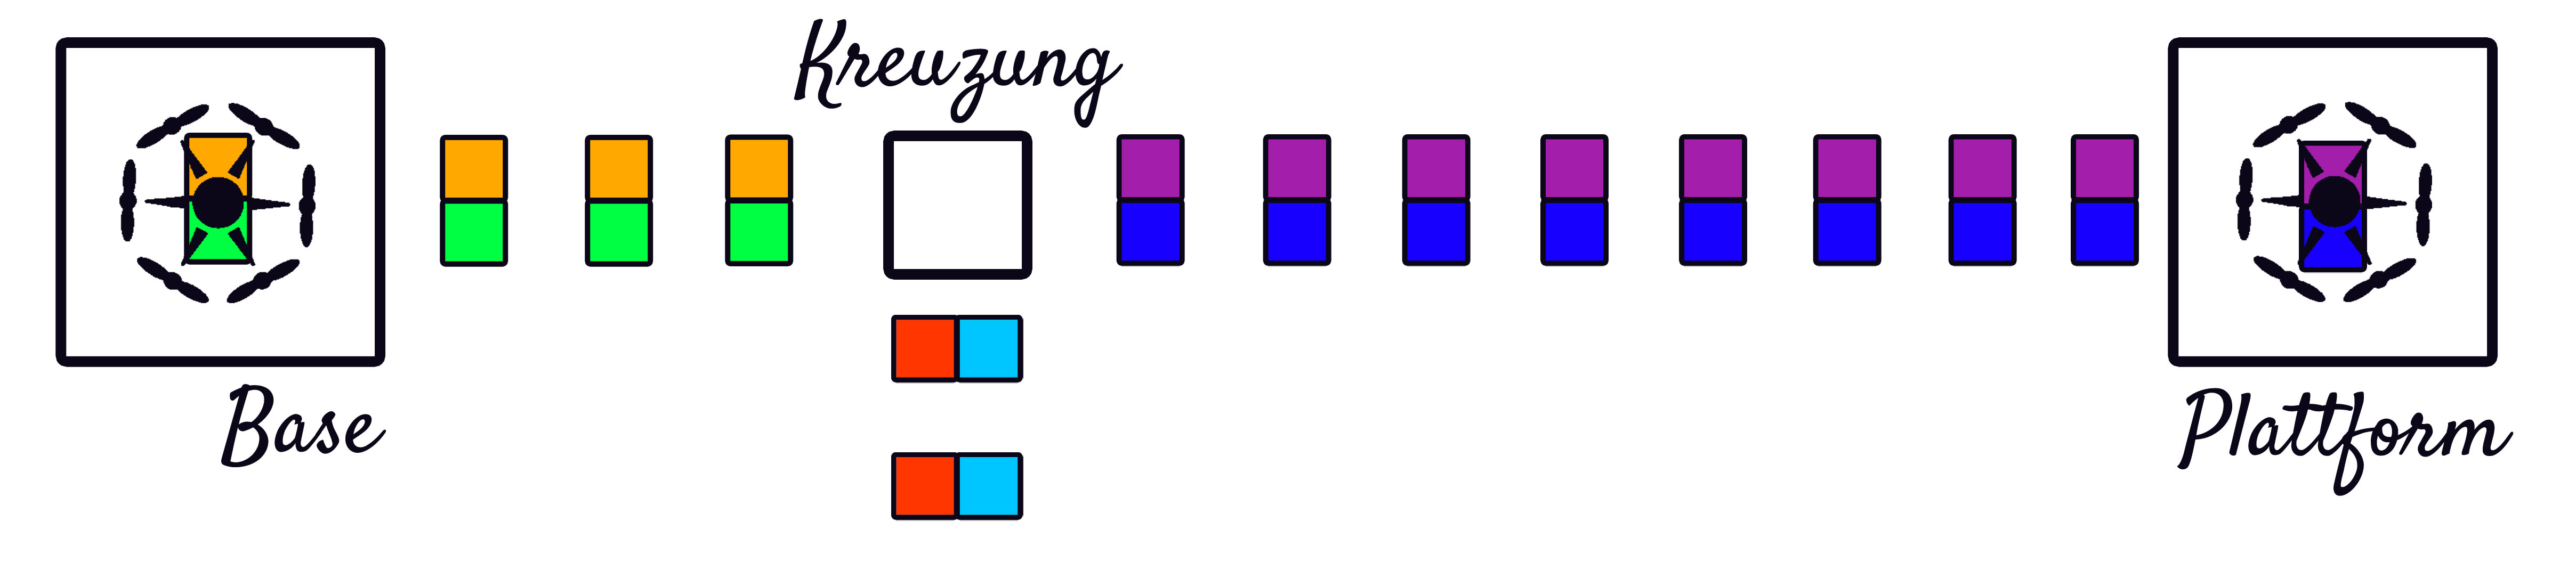
\includegraphics[width = \textwidth]{Bilder/bor_var1}
      \par\end{centering}
      \caption{Variante: Ein Farbcode pro Wegabschnitt}
      \label{Variante1}
    \end{figure}

  \subsection*{Farbcodes variieren}
  Das gewählte System wird ebenfalls mittels zweifarbiger Codes umgesetzt, der Unterschied zum vorigen System liegt in der Variation der Farbcodes. Es dürfen keine gleichen Farbcodes nebeneinander liegen, da die relative Position auf diese Weise besser bestimmt werden kann. Es besteht keine Verwechslungsgefahr mit einem anderen Farbcode. Außerdem kann durch die Anzahl der Farbcodes jeder Farbcode genau zugeordnet werden, der letzte Farbcode kann so einfach erkannt werden und das erleichtert den Landevorgang. Ein Nachteil des Systems ist der Mehraufwand im jeweiligen Restaurant, da die Farbcodes in einer bestimmten Reihenfolge aufgelegt werden.

      \begin{figure}[H]
      \begin{centering}
        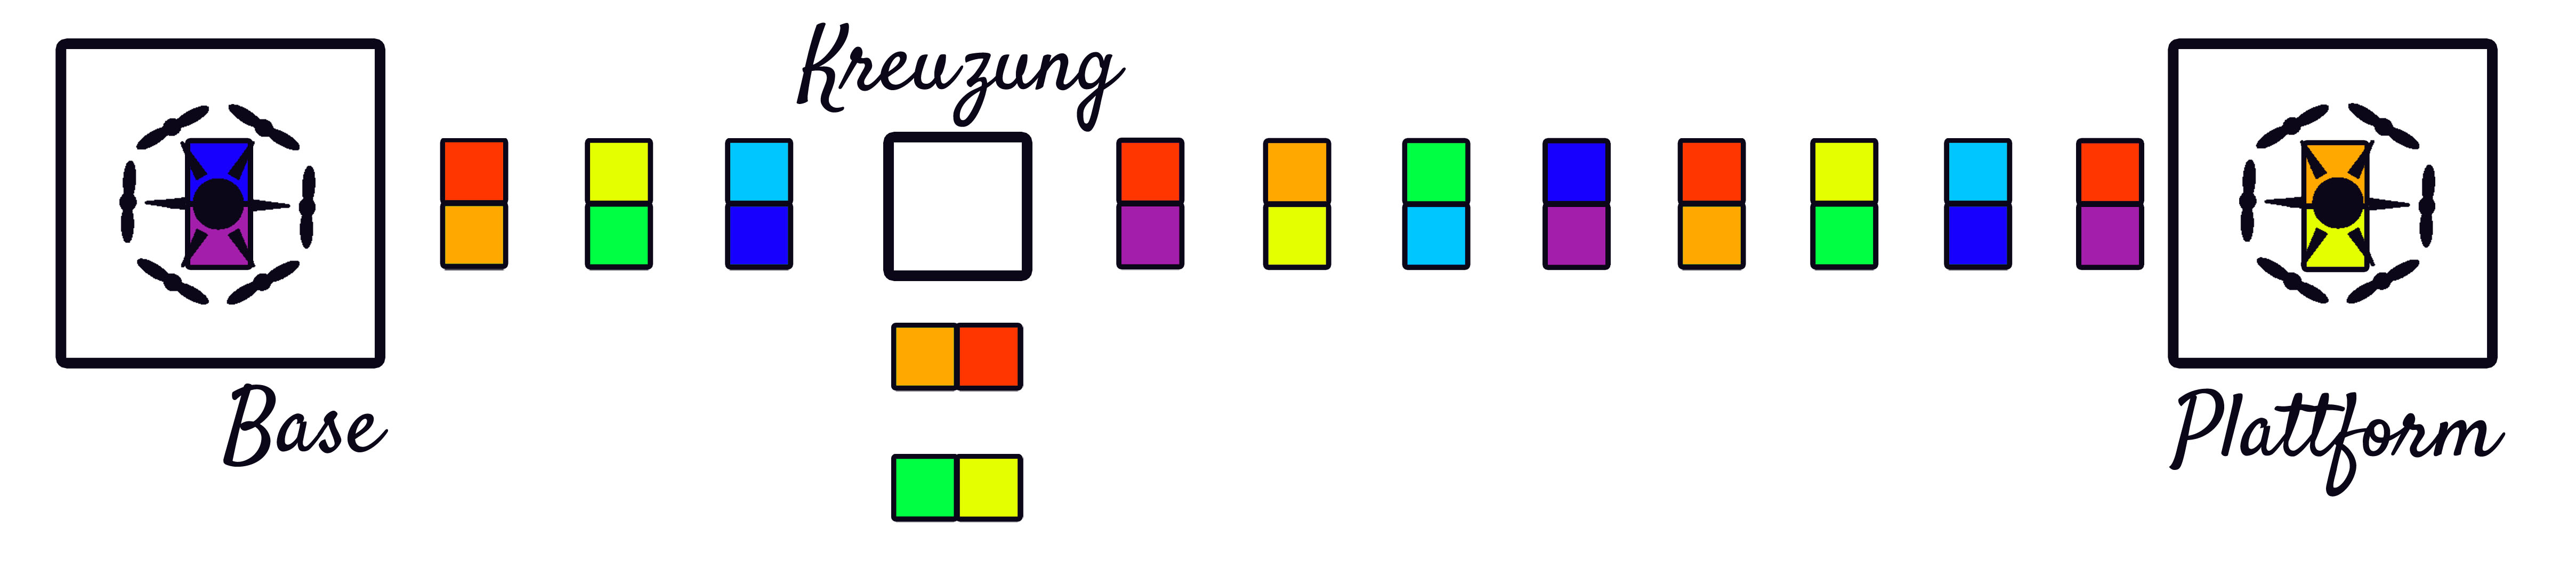
\includegraphics[width = \textwidth]{Bilder/bor_var2}
      \par\end{centering}
      \caption{Variante: Farbcodes variieren}
      \label{Variante2}
    \end{figure}

  \subsection*{Tracking mittels Infrarot}
  Um das System auch ohne entsprechende Lichtverhältnisse durchführen zu können, besteht die Möglichkeit einen Infrarotfilter an der Pixycam anzubringen und die Wegpunkte mittels Infrarotlampen zu markieren. Das System kann dadurch auch im Dunkeln angewendet werden, aktive Marker benötigen dafür einen Stromanschluss, da sie infrarotes Licht an den Empfänger senden. Bei passiven Markern, werden Infrarotlampen am Hexacopter benötigt, um das Licht reflektierender Marker zu empfangen.

  \subsection{Das gewählte Konzept}
  Das gewählte Konzept ist eine hybride Methode zwischen optischem Tracking und einer Laufzeitmessung mit akustischen Wellen.
  Durch die Pixy CMUcam5 werden am Boden liegende Farbcodes getrackt. Diese variieren, um die relative Position besser bestimmen zu können. Mit der Information, über welchem Farbcode sich der Hexacopter befindet, kann die Position im zweidimensionalen Raum herausgefunden werden. Da der Hexacopter fliegt, muss das System dreidimensional sein. Die z-Koordinate, beziehungsweise die Höhe, wird deswegen mit einem Ultraschallsensor über eine Laufzeitmessung bestimmt.

  Das System wurde auf die oben erklärten Eigenschaften analysiert:

  \subsection*{Physische und symbolische Positionierung}
  Die Positionierung erfolgt physisch. Durch die Pixy kann die tatsächliche Position ermittelt werden.
  Zum besseren Verständnis, werden die Positionen ebenfalls symbolisch beschrieben. Es werden die Namen Base, für die Küche beziehungsweise den Stützpunkt, Weg für die Route aus Colorcodes und Tisch, für die Landeplattform, auf der der Hexacopter landen soll, verwendet.

  \subsection*{Relative Positionierung}
  Das gewählte System gestaltet sich relativ, da der Hexacopter seine Position relativ zu Farbobjekten bestimmt.

  \subsection*{Selbstortendes Positionierungssystem}
  Das Positionierungssystem ist selbstortend. Die am Boden liegenden Farbobjekte werden von der Pixy getrackt und die daraus entstehenden Daten verarbeitet. Der Hexacopter kann ohne externe Einflüsse navigieren und ist somit unabhängig.

  \subsection*{Genauigkeit}
  Da das System mittels optischem Tracking umgesetzt wird, ist die Genauigkeit sehr hoch.
  Der verwendete Ultraschallsensor misst die Entfernung mit einer Messgenauigkeit von 3mm.

  \subsection*{Skalierung}
  Das System ist beliebig skalierbar, da es auf Farbcodes basiert. Es besteht die Möglichkeit, beliebig viele Farbcodes dem Weg hinzuzufügen oder wieder wegzunehmen. Die Routen sind im Adminbereich hinterlegt und müssen diese, je nachdem, wie der Administrator die Farbcodes legt, auch mitverändern. Im System gibt es aus Testgründen eine Grenze von 20 Farbcodes, diese kann aber einfach verändert werden.

  Die Pixy CMUcam5 ist in der Lage 135 Objekte pro Frame zu tracken. Unser System ist selbstortend und interessiert sich nur für ein Objekt pro Frame. \cite{PIXY_Porting}

  Das System ist, wegen des Ultraschallsensors auf eine Höhe von 3 Metern begrenzt. Im System ist eine Maximalhöhe von $\SI{220}{\centi\metre}$ über dem Boden und $\SI{120}{\centi\metre}$ über einem Tisch hinterlegt.

  \subsection*{Kosten}
  Da  die Positionierung auf einer Kamera mit Farbcodes, einem Ultraschallsensor, einem Mikrocontroller und einem WLAN-Modul sowie einem WLAN fähigen Gerät, als Admin-Interface, basiert, sind die Kosten sehr gering.

  \subsection*{Limitierung}
  Da die Pixy CMUcam5\cite{Pixy} ein optisches Trackingsystem ist, muss Sichtkontakt zwischen der Kamera und dem zu trackenden Objekt bestehen. Weiters müssen zuvor gespeicherte Farben wiedererkannt werden, die Lichtverhältnisse dürfen sich nicht verändern.
  Objekte müssen eine Mindestgröße von 4x1 Pixel in einem Frame ausmachen. Die Pixycam kann Objekte, laut Angaben der Website, über Kilometer tracken, wenn diese groß genug sind. Beispielsweise kann ein Objekt in Ping-Pong Ball Größe aus einer Entfernung von etwa 3 Metern gescannt werden. 

  Das System kann sowohl Indoor als auch Outdoor angewendet werden. Da die Farbobjekte am Boden positioniert werden, werden keine Wände, Decken oder sonstige Räumlichkeiten benötigt. Die genannten Objekte würden die Positionsbestimmung aber auch nicht beeinträchtigen.

  Der Ultraschallsensor eignet sich für den Bereich zwischen $\SI{2}{\centi\metre}$ und $\SI{3}{\metre}$. Bei der Entfernungsmessung muss man die Schallgeschwindigkeit berücksichtigen. Da diese temperaturabhängig \cite{Ultrasonic} ist, muss darauf geachtet werden, dass die Raumtemperatur in etwa der für die Entfernungsberechnung im Mikrocontroller verwendeten Temperaturkonstante entspricht. Bei 20 Grad Celsius beträgt diese 343 m/S. Wenn die Abweichung 20 Grad Celsius, in diesem Beispiel eine Temperatur von etwa 0 oder 40 Grad Celsius beträgt, kann ein Fehler von 3,4 Prozent erwartet werden.
  Bei der Reflektion auf glatten und ebenen Flächen erzeugt das beste Messergebnis, bei Distanzen unter $\SI{1}{\metre}$ erweisen sich beide Faktoren als unkritisch.
  Weiters muss der Winkel des Sensors beachtet werden, dabei spielt die Entfernung eine Rolle. Unter $\SI{1}{\metre}$ kann der Sensor bis zu 45 Grad geneigt sein, bei der maximalen Höhe von $\SI{3}{\metre}$ sind höchstens 15 Grad möglich.
